\chapter{Arrays of Arrays}

\section{Initializing Two-Dimensional Arrays}
You already know that you can initialize a one-dimensional array by putting the values in braces:

\begin{code}
int[] ages = {35, 27, 45, 58};
\end{code}

Because two-dimensional arrays are stored in Java as an array of arrays, as shown in Figure~\ref{fig:2D-array}, you can initialize them in a simliar manner.

\begin{figure}[!ht]
\begin{center}
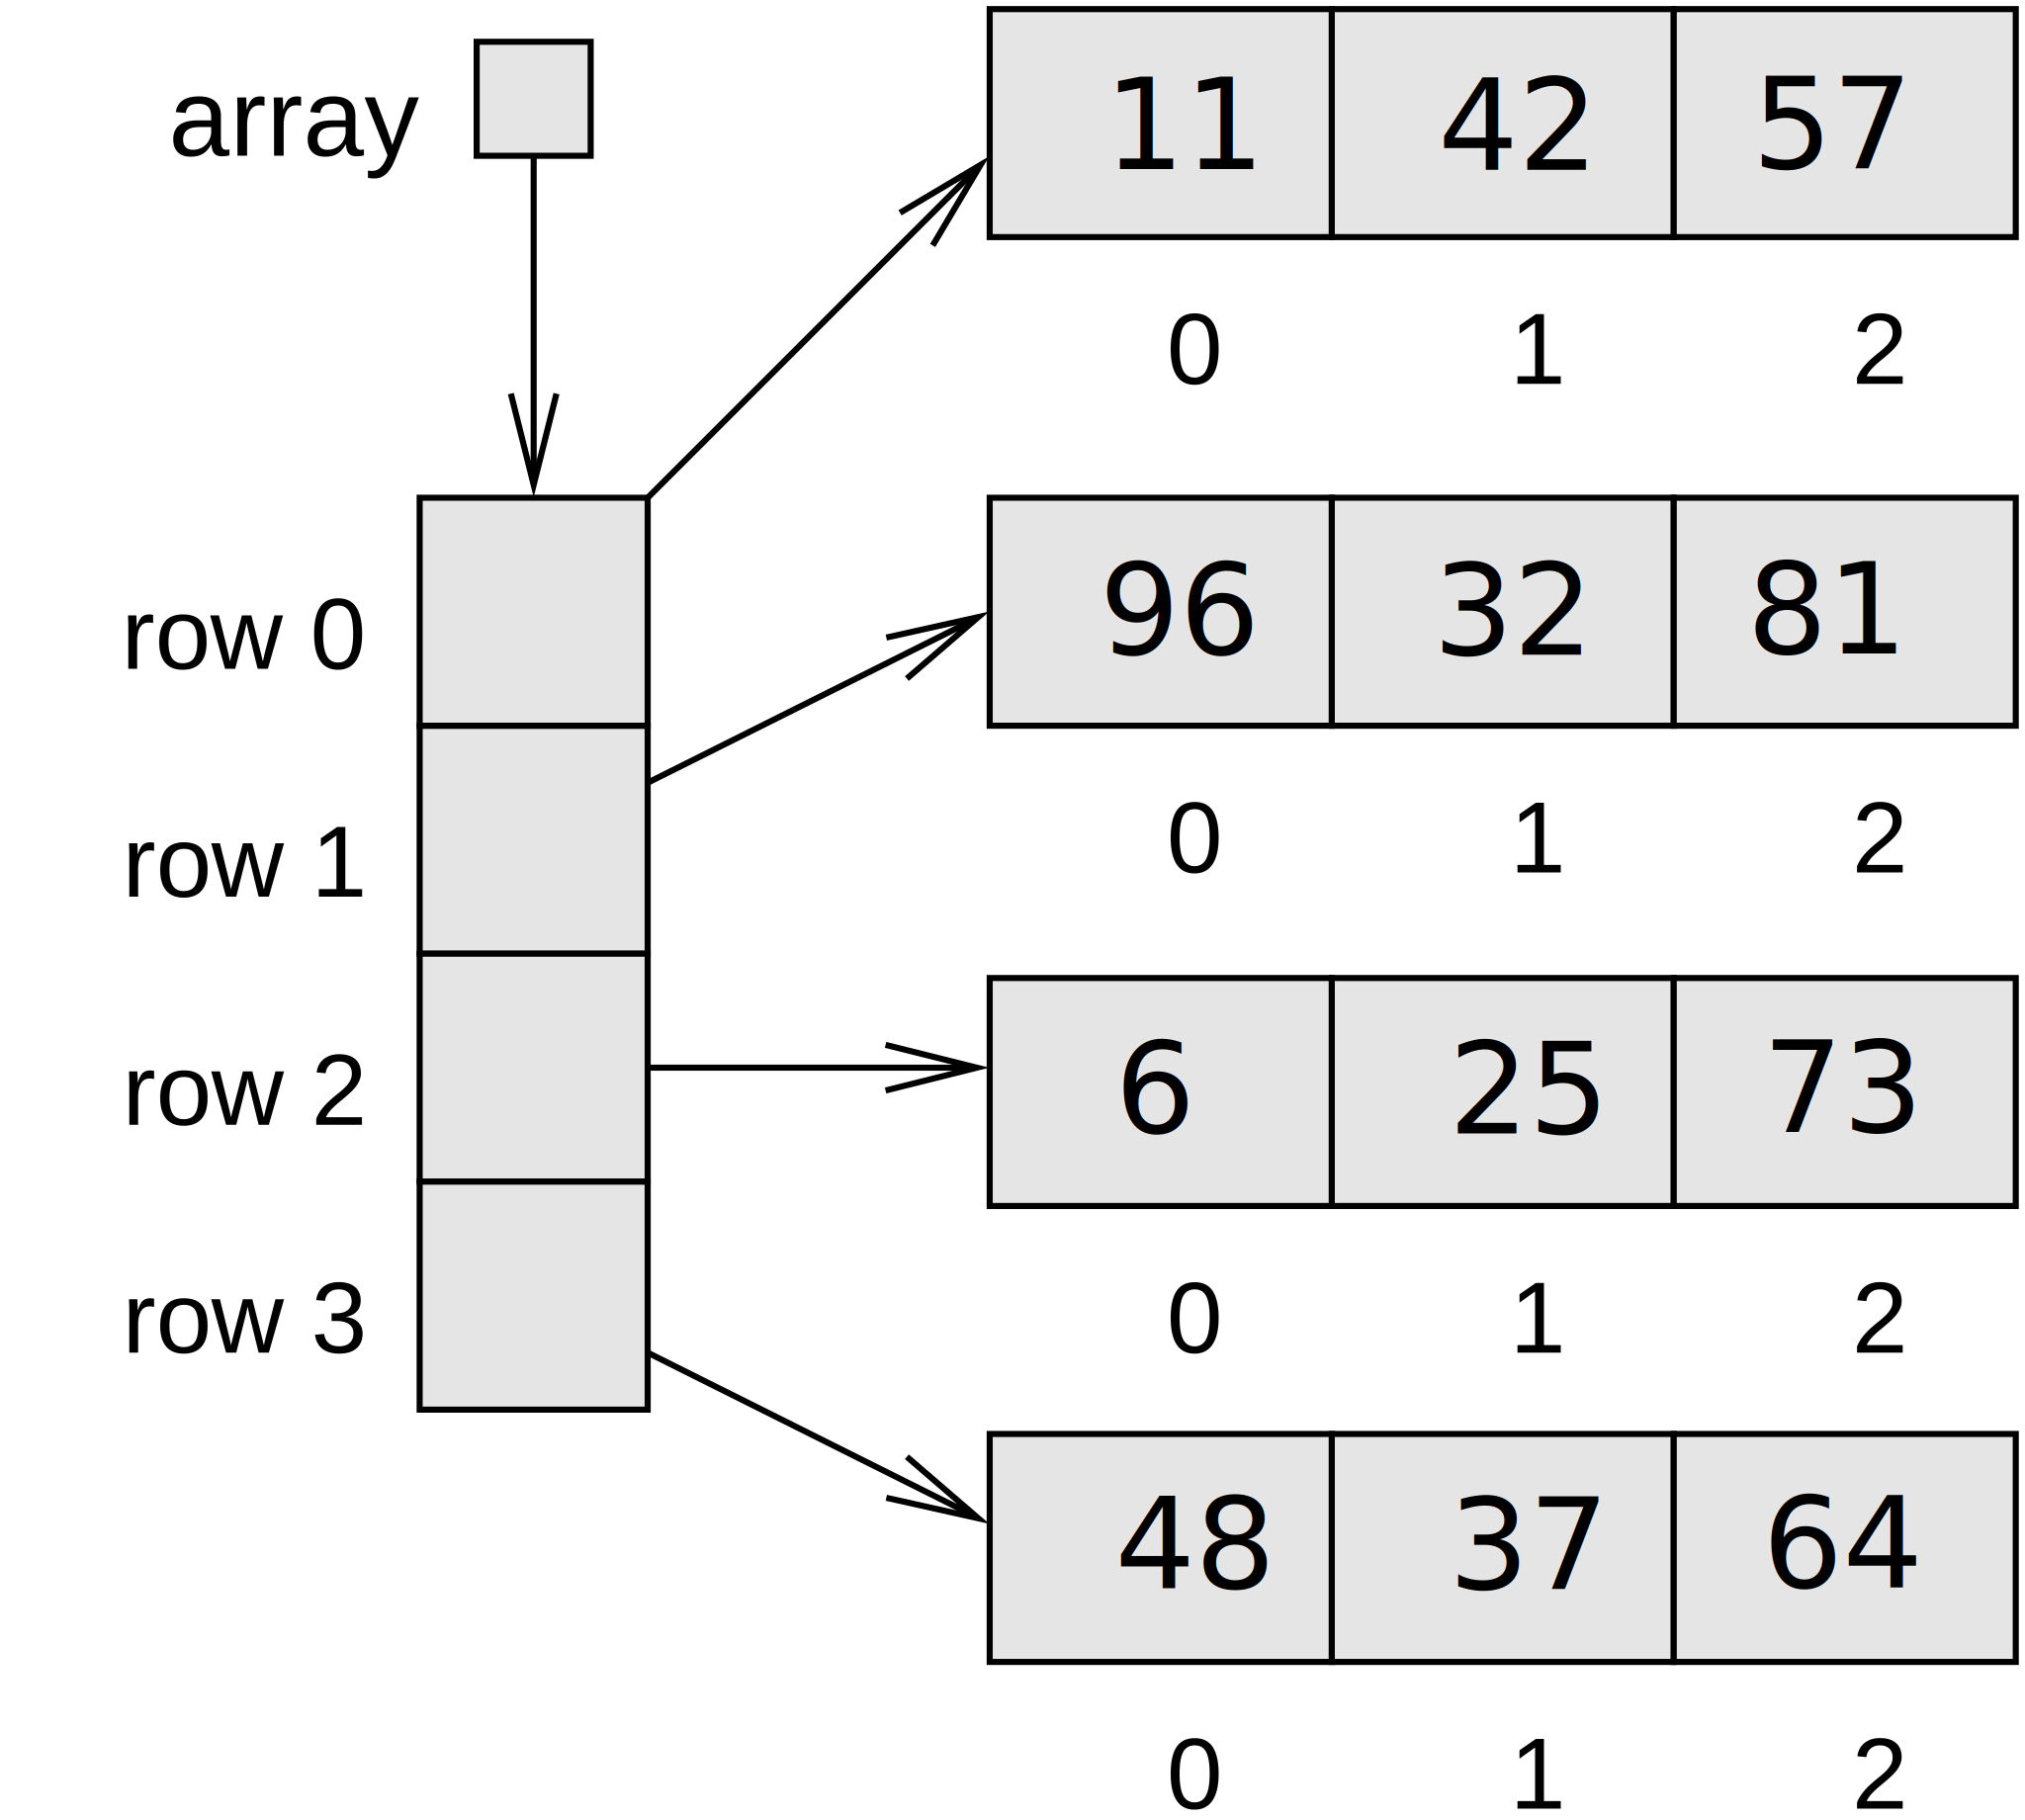
\includegraphics{figs/ch15/2D-array.pdf}
\caption{Storing rows and columns with a 2D array.}
\label{fig:2D-array} 
\end{center}
\end{figure}

\begin{code}
int[ ][ ] array = {
    {11, 42, 57},
    {96, 32, 81},
    { 6, 25, 73},
    {48, 37, 64}
};
\end{code}

However, there are times that we need to be able to read two-dimensional arrays from a user. It would be useful to have a small library of code that would allow us to read and print two-dimensional arrays so that we would not have to copy and paste the code into every program that needs it. That is the subject of the next section and the second exercise.

\section{Programs in Multiple Files}
Up to this point, all of our Java programs have been written in one file. We have used \java{import} to bring in classes and methods from other files.  Now it’s time to learn how to do this ourselves. There are many ways to structure a program so that it can be divided into separate files that are brought together at run time; the method we're using here is the simplest.

As an example, let's say we would like to have some methods that are generally useful for doing statistics with arrays of \java{double} values. We'll put them into a \java{public} class of their own. The following code gives the outline; you can download the entire file from the code repository at \url{https://github.com/jdeisenberg/ThinkJava2ExCode}

\begin{code}
public class ArrayStats {

    public static double mean(double[ ] data) {
        // calculation code goes here
        return result;
    }
    
    public static double stdv(double[ ] data) {
        // code goes here
        return result;
    }
}
\end{code}

You can now use these methods from another program, say, \java{TestStats.java} by putting the \java{ArrayStats.java} file in the same directory as the \java{TestStats.java} file.  If you do this, you don't need to do an \java{import}:

\begin{code}
public class TestStats {

    public static void main(String[ ] args) {
        double [ ] values = {10.0, 47.0, 6.6, 505.0217, 11.0};
        double avg = ArrayStats.mean(values);
        double stdDev = ArrayStats.stdv(values);
        System.out.printf("Average: %.3f\n", avg);
        System.out.printf("Standard Deviation: %.3f\n", stdDev);
    }
}
\end{code}

More complex ways of dividing a Java program into separate files involves the concepts of \java{package} and \java{module}. You can see documentation about this at \url{https://docs.oracle.com/javase/specs/jls/se9/html/jls-7.html}. 

\section{Exercises}

\begin{exercise}
Create a two-dimensional array of \java{int} that represents the following table of sales (in thousands of units), measured quarterly for three years. The first row and the leftmost column won't be part of your table; they are here to label the items properly so you can understand how the table is structured.

\begin{tabular}{|l|l|l|l|l|}
\hline
Year & Q1 & Q2 & Q3 & Q4 \\ \hline
1     & 27 & 24 & 29 & 28 \\ \hline
2     & 36 & 38 & 34 & 33 \\ \hline
3     & 34 & 39 & 37 & 36 \\ \hline
\end{tabular}

Then, have your program calculate and print:

\begin{itemize}
\item The total sales for each of the three years
\item The total sales for each quarter (across the three years)
\item The grand total of sales
\end{itemize}
\end{exercise}

\begin{exercise}
In this exercise, you'll write methods for doing input and output of a two-dimensional array. Put these methods into a file named \java{IO2D.java} (standing for Input/Output 2D). You will use these methods in the subsequent exercises.

{\bf Input}: Write a \java{public static double[ ][ ]} method named \java{getDoubleArray2D} with four parameters:

\begin{itemize}
\item A \java{Scanner} object
\item The prompt for the description of the array to enter (\java{String})
\item The number of rows (\java{int})
\item The number of columns (\java{int})
\end{itemize}

The method returns a two-dimensional array of \java{double}. For example, you might call it as:

\begin{code}
double [ ][ ] temps = getIntArray2D(input,
  "Enter temperature data one row at a time", 7, 3);
\end{code}

{\bf Output}: Write a \java{public static void} method named \java{printDoubleArray2D}, with two parameters:
\begin{itemize}
\item A formatting \java{String} like you would use in \java{System.out.printf} or \java{String.format}.
\item The array to be printed
\end{itemize}

This method will print out the arrays, using the given format for each element in the array. You might call it
like this:

\begin{code}
printDoubleArray2d(temps, "%.1f");
\end{code}

Then, in a class named \java{TestInputOutput}, write a \java{main} method that creates a 3 row, 4 column array of \java{double} and calls \java{getDoubleArray2D} and \java{printDoubleArray2D} to read an array and print it out. 

Here is sample output from this code:

\begin{code}
double[ ][ ] values = IO2D.getArray2d(input,
    "Enter three rows of data, one row at a time.", 3, 4);
System.out.println();
System.out.println("Here is your data:");
IO2D.printArray2d("%7.1f", values);
\end{code}

\begin{stdout}
Enter three rows of data, one row at a time.
Enter 4 items for row 1: 3.4 7.8 2.93 -12.1
Enter 4 items for row 2: 14.4 8.75 3.45 18.2225
Enter 4 items for row 3: 31.2 -56.4 19.21 47.66

Here is your data:
    3.4     7.8     2.9   -12.1 
   14.4     8.8     3.5    18.2 
   31.2   -56.4    19.2    47.7 
\end{stdout}

\end{exercise}

\begin{exercise}
In this exercise and the following exercises, you will develop methods that do mathematics with two-dimensional arrays, also called {\em matrices}.  Create a file named \java{MatrixMath.java}, which will have a \java{public class MatrixMath}.

First, write a method that adds two matrices. You do this by adding the corresponding entries of the two matrices:

\begin{equation*}
\begin{pmatrix}
1 & 2 & 3 \\
4 & 5 & 6 \\
7 & 8 & 9
\end{pmatrix}
+
\begin{pmatrix}
10 & 11 & 12 \\
13 & 14 & 15 \\
16 & 17 & 18
\end{pmatrix}
\rightarrow
\begin{pmatrix}
11 & 13 & 15 \\
17 & 19 & 21 \\
23 & 25 & 27
\end{pmatrix}
\end{equation*}

Here is the signature of the method:

\begin{code}
public static double[][] add(double[][] arr1, double[][] arr2)
\end{code}

The two arrays must have the same number of rows and columns. Write a method named \java{isAddCompatible} that will do that test for the users of your code. The method returns \java{true} if the arrays can be added, \java{false} otherwise. Its signature is:

\begin{code}
public static boolean isAddCompatible(double[][] arr1, double[][] arr2)
\end{code}

To test these methods, write a separate file with a \java{main} method that:

\begin{itemize}
\item Asks the user for the dimensions of one array and reads it in.
\item Asks the user for the dimensions of another array and reads it in.
\item If the arrays are compatible, add them and print the resulting array. If not, print an appropriate error message.
\end{itemize}

\end{exercise}

\begin{exercise}
Add a method to the \java{MatrixMath} class:

\begin{code}
public static double[][] scale(double[][] arr, double factor)
\end{code}

This method returns a new array the same size as the input array, with each element in the array multiplied by the given factor. Write a test program in a separate file that asks the user for the dimensions of an array, reads it in, asks for a scaling factor, reads that in, and scales the elements by the given factor and prints the result.
\end{exercise}

\begin{exercise}
Add a method to the \java{MatrixMath} class that returns the {\em transpose} of an array. When you transpose an array, the first row becomes the first column, the second row becomes the second column, etc. For example:

\begin{equation*}
\begin{pmatrix}
1 & 2 & 3 & 4 \\
5 & 6 & 7 & 8 \\
9 & 10 & 11 & 12
\end{pmatrix}
\rightarrow
\begin{pmatrix}
1 & 5 & 9 \\
2 & 6 & 10 \\
3 & 7 & 11 \\
4 & 8 & 12
\end{pmatrix}
\end{equation*}

The header of the method is:

\begin{code}
public static double[][] transpose(double[][] arr)
\end{code}


Write a test program in a separate file that asks the user for the dimensions of an array, reads it in, transposes it, and prints the result.

\end{exercise}

\begin{exercise}
Adding matrices is fairly straightforward. Multiplying them is anything but! In this exercise, you will write a method to multiply two matrices. The header of the method is:

\begin{code}
public static double[][] multiply(double[][] a, double [][] b)
\end{code}

To multiply a matrix $a$ by matrix $b$, the number of columns in $a$ must be the same as the number of rows in $b$, and the two matrices must have elements of the same or compatible types. Let $c$ be the result of the multiplication. Assume that $a$ has $n$ columns. Each element $c_{ij}$ is $a_{i1} \times b_{1j} + a_{i2} \times b_{2j} + ... + a_{in} \times b_{nj}$. For example,

\begin{align*}
\begin{pmatrix}
1 & 2 & 3 \\
4 & 5 & 6 \\
\end{pmatrix}
\times
\begin{pmatrix}
7 & 10 \\
8 & 11 \\
9 & 12
\end{pmatrix}
=
\end{align*}
%
% PDFLatex doesn't seem to like splitting into lines
% if I add a blank line; it gives errors. Hence
% I have to start a new equation.
%
\begin{align*}
\begin{pmatrix}
1\cdot 7+2\cdot 8+3\cdot 9 & 4\cdot 7+5\cdot 8+6\cdot 9\\
1\cdot 10+2\cdot 11+3\cdot 12 &  4\cdot 10+5\cdot 11+6\cdot 12\\
\end{pmatrix}
=
\begin{pmatrix}
50 & 68\\
122 & 167
\end{pmatrix}
\end{align*}

Implement a method with this header:

\begin{code}
public static boolean isMultiplyCompatible(double [][] arr1,
    double [][] arr2)
\end{code}

This will return \java{true} if the number of columns in \java{arr1} is equal to the number of rows in \java{arr2}, \java{false} otherwise.

Your \java{main} method will prompt the user for the number of rows and columns for the first matrix, then its contents. It will then prompt the user for the number of rows and columns for the second matrix, then its contents. It will then determine if the matrices are compatible by calling \java{isMultiplyCompatible}. If the matrices are compatible, the program will call the \java{multiply} method and print the returned matrix. If not, it will print an appropriate error message.

Here is an example of a run of the program:

\begin{stdout}
Matrix A
Enter number of rows: 2
Enter number of columns: 3
Enter contents by rows: 1 2 3 4 5 6
Matrix B
Enter number of rows: 3
Enter number of columns: 2
Enter contents by rows: 7 10 8 11 9 12

Matrix C is
50.0 68.0 
122.0 167.0
\end{stdout}

\end{exercise}

\begin{exercise}
Write a program named {\em Dice.java} that will do the following:

\begin{enumerate}

\item Ask the user how many times they wish to roll a pair of dice, from 1-999. Validate the input---keep asking until the number is in range. Write a method named \java{getNRolls} to do this step. The method takes a \java{Scanner} object as its parameter and returns the number of rolls the user desires.

\item Create a $6 \times 6$ array named \java{rolls} to hold the result of the rolls.

\item Simulate randomly rolling a pair of dice as many times as the user requested. As you roll the dice, count how many times each combination of dice was rolled. For example, if the first die is a 3 and the second die is 5, you will add one to the entry at \java{rolls[2][4]}. (If you generate numbers in the range 1-6, you will have to subtract one at appropriate places. If you generate numbers in the range 0-5, you don't need to do any subtraction). Write a method named \java{rollDice} to do this step. It takes the number of rolls as its parameter and returns the two-dimensional array of \java{rolls}.

\item Print out the array, properly labeled, so that the numbers all line up. You can do this in \java{main} or write a method to do it.

\item Go through the array you created in step 3 and figure out how many times the dice totaled 2, 3, 4, \textellipsis 12. Write a method called \java{calcFrequencies} to do this. It will take the \java{rolls} array as its parameter and return a single-dimensional array of length 11, which your \java{main} method will store in an array named \java{totals}.

\item Print the frequency array from step 5, properly labeled. You may do this in \java{main} or write a method to do it.

\end{enumerate}

Yes; I know this is ``inefficient.'' It is possible to construct the \java{totals} array at the same time that you create the \java{rolls} array. You could do everything in \java{main} without any other methods. However, I want you to practice passing and returning arrays to and from methods, so I decided to write the exercise this way.

Sample output:

\begin{stdout}
How many times do you want to roll the dice (1-999)? 200
Frequencies for individual dice
      1   2   3   4   5   6
    ------------------------
1|    3   7   2   3   8   4
2|    4   7   2   5  10   5
3|    9  10   7   4   6   5
4|    6   4   5   7   4   8
5|    3   3   3   8   6   6
6|    5   5   8   7   3   8

Frequencies of totals
 2:   3
 3:  11
 4:  18
 5:  21
 6:  27
 7:  31
 8:  26
 9:  25
10:  21
11:   9
12:   8
\end{stdout}

\end{exercise}
